\documentclass[a4paper,12pt]{article}
\usepackage[utf8]{inputenc}
\usepackage[T1]{fontenc}
\usepackage{amsmath}
\usepackage{amsfonts}
\usepackage{amssymb}
\usepackage[version=4]{mhchem}
\usepackage{stmaryrd}
\usepackage{enumerate}
\usepackage{hyperref}
\usepackage{tikz}
\usetikzlibrary{positioning, shapes.geometric, arrows.meta, chains}
%\usepackage{tikzexternal}

% =======================================================================
% Margins --- save forests
\NeedsTeXFormat{LaTeX2e}
\oddsidemargin -10 pt       %   Left margin on odd-numbered pages.
\evensidemargin 10 pt       %   Left margin on even-numbered pages.
\marginparwidth 1 in        %   Width of marginal notes.
\oddsidemargin -1.5 true cm %   Note that \oddsidemargin = \evensidemargin
\evensidemargin -1.5 true cm
\marginparwidth 0.75 in
\textwidth 7.5 true in % Width of text line.
\textheight 26.0 true cm
\topmargin -2.5 true cm

% =======================================================================

\title{Programming Paradigms (Neapolis University Pafos)
  Assignment 3: Audio Processing System}

%\author{Alex Avdiushenko}
\date{April 2025}

\begin{document}
\maketitle

\begin{center}
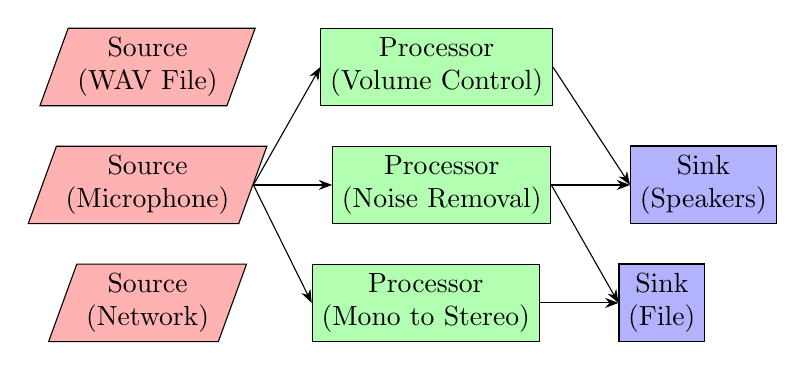
\begin{tikzpicture}[
    node distance = 5mm and 10mm,
    start chain = going right,
    box/.style = {rectangle, draw, on chain, align=center, fill=blue!30},
    process/.style = {rectangle, draw, on chain, align=center, fill=green!30},
    io/.style = {trapezium, trapezium left angle=70, trapezium right angle=-70, draw, on chain, align=center, fill=red!30}
]

% Pipeline 1
    \node[io] (source1) {Source\\(WAV File)};
    \node[process] (proc1) {Processor\\(Volume Control)};
    %\node[box] (sink1) {Sink\\(File)};

% Pipeline 2
    \node[io, below=of source1] (source2) {Source\\(Microphone)};
    \node[process, right=of source2] (proc2) {Processor\\(Noise Removal)};
    \node[box, right=of proc2] (sink2) {Sink\\(Speakers)};

% Pipeline 3
    \node[io, below=of source2] (source3) {Source\\(Network)};
    \node[process, right=of source3] (proc3) {Processor\\(Mono to Stereo)};
    \node[box, right=of proc3] (sink3) {Sink\\(File)};

% Arrows
    \draw[-Stealth] (source2.east) -- (proc1.west);
    \draw[-Stealth] (proc1.east) -- (sink2.west);
    \draw[-Stealth] (source2.east) -- (proc2.west);
    \draw[-Stealth] (proc2.east) -- (sink2.west);
    \draw[-Stealth] (proc2.east) -- (sink3.west);
    \draw[-Stealth] (source2.east) -- (proc3.west);
    \draw[-Stealth] (proc3.east) -- (sink3.west);
\end{tikzpicture}
\end{center}

\textbf{Set-up:} For this assignment, you will create a versatile audio processing
application in Java that can handle various transformations on audio streams,
such as volume adjustment, speed modification, noise removal, and channel manipulation
(mono/stereo). The system should be able to process input from WAV files,
microphone streams, and other sources.
Use provided \href{https://github.com/avalur/avalur.github.io/tree/master/cs_basics/oop_project}{Java-project blueprint} for reference.

\section{Considerations for OOP and Extensibility}
\begin{enumerate}
  \item \textbf{Encapsulation}: Keep system details hidden, exposing only what's necessary.
  \item \textbf{Inheritance}: Use abstract classes and interfaces to define and extend behaviors.
  \item \textbf{Polymorphism}: Leverage to allow different implementations of audio sources, processors, and consumers.
\end{enumerate}

This project challenges you to think about complex system design,
data flow, and the practical application of OOP principles
in a real-world scenario, using Java.
It's a great opportunity to explore advanced programming concepts,
software architecture, and audio processing techniques.

\section{Core Components and Design Approach}
\subsection{Audio Stream Abstraction: Interface}
\begin{enumerate}
    \item \textbf{Purpose}: Represent a generic audio stream, allowing
    for different implementations (file, microphone, network).
    \item \textbf{Key Methods}: `read()`, `write()`, `close()`.
\end{enumerate}
This interface forms the foundation for any class that aims to handle audio data within the system,
ensuring that basic operations like reading, writing, and closing are consistently implemented across various audio sources and destinations.
Implementing classes will provide the specifics of these operations based on the actual source or destination (e.g., file system, microphone hardware, network connection).

Next steps would involve creating concrete implementations of this interface for different audio sources and sinks,
such as a FileAudioStream for reading from and writing to audio files, MicrophoneAudioStream for capturing audio from a microphone,
or NetworkAudioStream for receiving and sending audio data over the network.

\subsection{Audio Processor Framework}
\begin{enumerate}
  \item \textbf{Purpose}: Define a framework for various audio processing algorithms (volume control, acceleration, mono/stereo conversion, noise removal, cutting/adding segments).
  \item \textbf{Design}: Use the Strategy pattern to allow for interchangeable algorithms that can be applied to audio streams.
\end{enumerate}

This framework allows you to easily extend the application with new audio processing algorithms
without modifying the existing codebase, adhering to the open/closed principle.
To add a new algorithm, you simply implement the AudioProcessingStrategy interface and
integrate it into the system by setting it as the current strategy in an AudioProcessingContext instance.

\subsection{Channel and Subchannel System}
\begin{enumerate}
  \item \textbf{Purpose}: Facilitate the flow of data between sources, processors, and consumers. Support subchannels for metadata, checksums, etc.
  \item \textbf{Design}: Implement a Channel class with capabilities to buffer data, manage subchannels, and connect to source and sink pins.
\end{enumerate}

\subsubsection*{Key Features}
\begin{enumerate}
  \item Audio Data Buffering: The main audio data buffer uses a BlockingQueue to store audio data bytes, enabling asynchronous data flow between components. The BlockingQueue handles thread-safe data exchange and synchronization.
  \item Subchannel Management: Subchannels are managed in a map, allowing for dynamic creation and usage. Each subchannel has its own BlockingQueue for buffering, suitable for different types of data, such as metadata or checksums.
  \item Thread-Safe Operations: The add and take operations for both main audio data and subchannel data are thread-safe, ensuring that data can be added and retrieved reliably in a concurrent environment.
\end{enumerate}

This design lays the groundwork for a flexible data flow system in your audio processing application,
supporting complex operations such as metadata management, error checking through checksums,
and asynchronous processing. The use of blocking queues for buffering also helps in managing flow control,
reducing the risk of data loss or overflow in high-throughput scenarios.

\subsection{Data Source and Consumer}
\begin{enumerate}
  \item \textbf{Data Sources}: Implementations for reading from WAV files, microphone input, and network streams.
  \item \textbf{Data Consumers}: Implementations for writing processed audio to files, sending over the network, or outputting to speakers.
\end{enumerate}

\subsubsection*{WAVFileReader}
This component reads audio data from a WAV file using `AudioSystem.getAudioInputStream` and sends the data to a specified channel.
It uses a buffer to read chunks of data and then sends these chunks through the channel.
It's essential to handle various exceptions that might occur during file reading and audio processing.

\subsubsection*{FileWriter}
This component listens for audio data from a channel and writes it to a file.
It uses a `FileOutputStream` for writing data. The loop continuously listens for data from the channel,
assuming an external mechanism to stop the loop (like a signal or specific data indicating the end of the stream).

Both components interact with the `Channel` class designed earlier,
showcasing how data sources and consumers can be implemented to work within an audio processing system.
These examples are simplified and might need additional considerations for error handling, synchronization,
and performance optimization in a real application.

\subsection{Pins and Handlers}
\begin{enumerate}
  \item \textbf{Purpose}: Define connection points for channels to sources,
  processors, and consumers. Handlers manage data flow and transformations.
  \item \textbf{Design}: Utilize the Observer pattern for dynamic data flow control and processing.
\end{enumerate}

\subsubsection*{Integration and Flow Control}
In this design, `ObservableChannel` acts as the subject, notifying its observers
(`DataPin` implementations) about new data.
`AudioProcessorPin` serves as an observer and handler for data processing,
utilizing a specified `AudioProcessingStrategy`.
This setup allows for flexible and dynamic data flow control within the audio processing system,
adhering to the Observer pattern.

The system can be extended with more pins and handlers for different processing or output needs,
showcasing the Observer pattern's power in creating a modular and extensible architecture.

\subsection{Utility Components}
\begin{enumerate}
  \item \textbf{Converters}: Can be used in processing pins or as standalone processing units
  depending on whether you're implementing STT, TTS, or other conversion functionalities.
  \item \textbf{Config Management}: For setting up and managing system configurations,
  potentially through visual representation using JavaFX. The JavaFX user interface (UI)
  can serve as the central hub for adjusting system settings and configurations, enhancing user interaction.
  \item \textbf{Logging and Debugging}: Integrated logging for monitoring system operations
  and aiding in debugging.
\end{enumerate}

By incorporating these utility components, the audio processing system becomes more robust,
user-friendly, and easier to maintain and debug.

\section{Choosing framework for Java application}
You have to choose a framework for developing Java applications,
especially for enterprise-level development.
In this project we use \textbf{Spring Framework},
a comprehensive framework, which provides a wide range of features such as dependency injection,
aspect-oriented programming, transaction management, and more,
facilitating the creation of high-performing, reusable code.

\subsection{Alternatives to Spring Framework}
Several frameworks offer similar functionality to Spring, each with its own strengths and focus areas.
Here are a few notable ones:
\begin{enumerate}
    \item \textbf{Micronaut}: A modern, JVM-based, full-stack framework for building modular,
    easily testable microservice and serverless applications.
    It's designed to be lightweight and fast, with minimal memory footprint and startup time, making it an excellent choice for microservices.
    \item \textbf{Quarkus}: Known as a Kubernetes-native Java stack,
    Quarkus is tailored for Java virtual machines (JVMs) and native compilation,
    optimizing Java specifically for containers and enabling it to become an effective platform
    for serverless, cloud, and Kubernetes environments.
    \item \textbf{Helidon}: Developed by Oracle, Helidon is a collection of Java libraries
    for writing microservices that run on a fast web core powered by Netty.
    It offers two programming models: Helidon SE, a reactive model, and Helidon MP,
    an implementation of MicroProfile for a more declarative style of programming akin to Spring.
    \item \textbf{Vert.x}: A tool-kit for building reactive applications on the JVM.
    It's event-driven and non-blocking, which means applications can handle
    a lot of concurrency using a small number of kernel threads.
    Vert.x lets you write applications in a variety of languages, not just Java.
    \item \textbf{Dropwizard}: A lightweight framework that lets you quickly build RESTful
    web services. It bundles together popular libraries like Jetty, Jersey, and Jackson,
    with a focus on providing you with everything you need to develop production-ready
    web services in a straightforward, no-fuss package.
\end{enumerate}

\section{The Problems (Finally)}
Note: we reserve the opportunity for reviewers to deduct points
for incomprehensible code or a carelessly designed project.
\begin{enumerate}
  \item \textbf{(20 points)} Implement a few sources and consumers,
  and create a working example of audio processing.

  \item \textbf{(30 points)} Write unit and integration tests for each component.

  \item \textbf{(30 points)} Integrate JavaFX or some other Java library you like
  for configuration and visualization, make nice UI.

  \item \textbf{(20 points)} Incorporate utility components like other converters,
  item loggers, and debug tools.

  \item (Lack Of) Challenge Problem:
  the most educational challenge problem is not something
  we can reasonably auto-grade or peer assess, so we encourage doing it even
  though it will not count toward your grade:
  Make a second version of your solution in a different OOP language:
  it may be Kotlin, Scala, Rust or even C#.
\end{enumerate}

\end{document}